\documentclass[thesis.tex]{subfiles}

\begin{document}
Once the ground state energy and the effective Hamiltonian have been calculated, any further properties of the ground state can be calculated using the correlated wave function written as an expansion of Slater determinants in the form of Eqn.\ \eqref{eq:cc_ansatz}.  However, many of the most interesting processes in nuclear physics involve excited-state properties.  Additionally, because the coupled cluster method requires a doubly closed-shell reference state, most topics in nuclear physics that can benefit from an \emph{ab initio} description are unreachable with the standard coupled cluster approach alone.

These restrictions motivate a class of techniques known as the \textit{equations-of-motion} (EOM) methods \cite{ROWE1968}.  Applied with the CC effective Hamiltonian, the \textit{equation-of-motion coupled cluster} (EOM-CC) method begins with a standard CC calculation of a closed-shell ground state.  Then, EOM \textit{target states} are built onto the correlated ground-state wave function in the same way that CI states were built from the reference state, Eqn.\ \eqref{eq:ci_expansion}.  Unfortunately, because the CCSD similarity transformation only decouples the ground state from $\ph{1}{1}$ and $\ph{2}{2}$ excitations, these target states are still coupled to each other.  Therefore, capturing the relevant correlations to describe EOM states involves a CI-like diagonalization of the effective Hamiltonian.


\section{Equation-of-Motion States} \label{section:eom_target_states}

The CC equations-of-motion states are built by applying a particular type of excitation operator to the correlated ground-state wave function in the same way that the correlated ground-state wave function was built by applying the exponential cluster operator to the reference state,
\begin{equation}\label{eq:eom_def}
  \ket{\Psi_{\mu}} = \Rop_{\mu}\corrket = \Rop_{\mu}\E^{\Top}\refket.
\end{equation}
The EOM excitation operator can be written as a linear combination of strings composed of particle creation operators and hole annihilation operators in increasing order, $\Rop_{\mu} = \RopB{0}_{\mu} + \RopB{1}_{\mu} + \RopB{2}_{\mu} + \cdots$.  The form of these strings is determined by the structure of the desired target state.  For example, excited states maintain the particle number of the reference state and ground state so that the constituent operator strings are $\ph{k}{k}$ operators.  The $A$-particle excited-state EOM operator $\Rop^{A}_{\mu}$ is,
\begin{equation}
  \Rop^{A}_{\mu} = \rint{\mu}{}{0} + \sum_{ai}\rint{\mu}{a}{i}\normord{\co{a}\ao{i}} + \frac{1}{4}\sum_{abij}\rint{\mu}{ab}{ij}\normord{\co{a}\co{b}\ao{j}\ao{i}} + \cdots,
\end{equation}
where $\RopB{0}_{\mu} = \rint{\mu}{}{0}$ represents the ground-state component of an excited state with the same conserved quantum numbers and the matrix elements, $\rint{\mu}{a}{i}, \rint{\mu}{ab}{ij}, \cdots$, are the normal-ordered components of $\Rop_{\mu}$.

In addition to excited states, particle-attached (PA) states can be reached by applying strings of the form $\mathrm{p,pph,ppphh,}$ etc. to the ground state.  These operator strings increase the number of particles by one and gives the \textit{particle-attached equation-of-motion} PA-EOM operator $\Rop^{A+1}_{\mu} = \RopB{1}^{A+1}_{\mu} + \RopB{2}^{A+1}_{\mu} + \cdots $,
\begin{equation} \label{eq:pa_right}
  \Rop^{A+1}_{\mu} = \sum_{a}\rint{\mu}{a}{}\normord{\co{a}} + \frac{1}{2}\sum_{abi}\rint{\mu}{ab}{i}\normord{\co{a}\co{b}\ao{i}} + \cdots.
\end{equation}
Lastly, particle-removed (PR) states can be reached by applying strings of the form $\mathrm{h,hhp,hhhpp,}$ etc. to the ground state.  These operator strings decrease the number of particles by one and give the \textit{particle-removed equation-of-motion} PR-EOM operator $\Rop^{A-1}_{\mu} = \RopB{1}^{A-1}_{\mu} + \RopB{2}^{A-1}_{\mu} + \cdots $,
\begin{equation} \label{eq:pr_right}
  \Rop^{A-1}_{\mu} = \sum_{i}\rint{\mu}{}{i}\normord{\ao{i}} + \frac{1}{2}\sum_{aij}\rint{\mu}{a}{ij}\normord{\co{a}\ao{j}\ao{i}} + \cdots.
\end{equation}

With these target states, the Schr\"odinger equation can be written by applying the Hamiltonian to Eq.\ \eqref{eq:eom_def},
\begin{gather}
  \Ham\ket{\Psi_{\mu}} = E_{\mu}\ket{\Psi_{\mu}}, \notag \\
  \Ham\Rop_{\mu}\E^{\Top}\refket = E_{\mu}\Rop_{\mu}\E^{\Top}\refket
\end{gather}
This equation can be written in terms of the effective Hamiltonian by multiplying with the operator $\E^{-\Top}$,
\begin{equation} \label{eq:eom_schrodinger}
  \E^{-\Top}\Ham\Rop_{\mu}\E^{\Top}\refket = E_{\mu}\E^{-\Top}\Rop_{\mu}\E^{\Top}\refket.
\end{equation}
Because both $\Rop_{\mu}$ and $\Top$ are excitation operators, containing only particle creation operators and hole annihilation operators, no nonzero contractions can occur between them (see section \ref{section:wicks_theorem}).  This means that the order of the two operators is inconsequential such that they commute with each other ($\Rop_{\mu}\Top = \Top\Rop_{\mu}$), which is also true for the exponential cluster operator ($\Rop_{\mu}\E^{\Top} = \E^{\Top}\Rop_{\mu}$).  This property can be used to rewrite Eq.\ \eqref{eq:eom_schrodinger} in terms of the effective Hamiltonian,
\begin{align} \label{eq:eom_schrodinger1}
  \E^{-\Top}\Ham\E^{\Top}\Rop_{\mu}\refket &= E_{\mu}\E^{-\Top}\E^{\Top}\Rop_{\mu}\refket \notag \\
  \EHam\Rop_{\mu}\refket &= E_{\mu}\Rop_{\mu}\refket.
\end{align}
Using the normal-ordered Hamiltonian, the equation can be rewritten as,
\begin{equation} \label{eq:eom_schrodinger2}
  \EHamN\Rop_{\mu}\refket = \Ecorr_{\mu}\Rop_{\mu}\refket.
\end{equation}

Up to this point, extending the CC method from the ground state to excited and open-shell states amounts to an energy eigenvalue problem involving the normal-ordered effective Hamiltonian and the EOM excitation operators $\Rop_{\mu}$.  The signature component of EOM methods is reached by multiplying the normal-ordered ground-state Schr\"odinger equation, Eq.\ \eqref{eq:normal_schrodinger}, with $\Rop_{\mu}$ and subtracting the result from Eq.\ \eqref{eq:eom_schrodinger2},
\begin{equation} \label{eq:eom_schrodinger3}
  \left(\EHamN\Rop_{\mu} - \Rop_{\mu}\EHamN\right)\refket = \left(\Ecorr_{\mu} - \Ecorr\right)\Rop_{\mu}\refket.
\end{equation}
The right-hand side of this equation can be rewritten as the commutator $\left[ \EHamN,\Rop_{\mu} \right]$ and the energy difference can be defined as $\omega_{\mu} \equiv \Ecorr_{\mu} - \Ecorr$ so that the fundamental EOM equation is,
\begin{equation} \label{eq:eom_schrodinger4}
  \left[ \EHamN,\Rop_{\mu} \right]\refket = \omega_{\mu}\Rop_{\mu}\refket.
\end{equation}
The name \textit{equation-of-motion} refers to the resemblance of this equation with the commutator-based Heisenberg representation of quantum mechanics.  The objective behind this formulation is to reduce the dependence of EOM states on the ground state by removing common terms between them.  This reduction is accomplished by noticing that, like the commutator between $\EHamN$ and $\Rop_{\mu}$, the commutator between uncontracted terms of $\left[ \EHamN,\Rop_{\mu} \right]$ vanishes.  This simplifies the commutator in Eq.\ \eqref{eq:eom_schrodinger4} to only connected terms just as the effective Hamiltonian was simplified in Eq.\ \eqref{eq:cc_heff1},
\begin{equation} \label{eq:eom_schrodinger4}
  \left( \EHamN\Rop_{\mu} \right)_{\mathrm{c}}\refket = \omega_{\mu}\Rop_{\mu}\refket.
\end{equation}

Equation\ \eqref{eq:eom_schrodinger} constitutes a generalized eigenvalue problem which solves for the components of the EOM operator, $\rint{\mu}{}{}$, and the energy difference, $\omega_{\mu}$.  If only the energy of excited or open shell states are required, solving this equation is sufficient for such a task.  However, computing properties of EOM states requires the Hermitian conjugate of the EOM operator $\Rop^{\dagger}_{\mu}$, and as encountered before, the non-Hermiticity of the effective Hamiltonian complicates this effort.


\section{Dual Solutions} \label{section:eom_dual}

Because the CC effective Hamiltonian is non-Hermitian ($\EHamN^{\dagger} \neq \EHamN$), the eigenvalue problem in Eq.\ \eqref{eq:eom_schrodinger2} has a corresponding left-eigenvalue problem,
\begin{equation} \label{eq:eom_dual1}
  \refbra\Lop_{\mu}\EHamN = \refbra\Lop_{\mu}\Ecorr_{\mu}.
\end{equation}
The operators $\Lop_{\mu}$ are de-excitation operators analogous to the corresponding right operators $\Rop_{\mu}$.  The left EOM operator for particle-attached states has the form,
\begin{equation} \label{eq:pa_left}
  \Lop^{A+1}_{\mu} = \sum_{a}\lint{\mu}{}{a}\normord{\ao{a}} + \frac{1}{2}\sum_{abi}\lint{\mu}{i}{ab}\normord{\co{i}\ao{b}\ao{}} + \cdots,
\end{equation}
and the left EOM operator for particle-removed states has the form,
\begin{equation} \label{eq:pr_left}
  \Lop^{A-1}_{\mu} = \sum_{i}\lint{\mu}{i}{}\normord{\co{i}} + \frac{1}{2}\sum_{aij}\lint{\mu}{ij}{a}\normord{\co{i}\co{j}\ao{a}} + \cdots.
\end{equation}
Again, the matrix elements $\lint{\mu}{}{}$ are the normal-ordered components of $\Lop_{\mu}$ and map to a corresponding $\rint{\mu}{}{}$.  Because there is not a corresponding left eigenvalue problem for the ground state in the form of Eq.\ \eqref{eq:normal_schrodinger}, the EOM eigenvalue problem for $\Lop_{\mu}$ cannot be reduced to the form of Eq.\ \eqref{eq:eom_schrodinger4}.  This amounts to calculating additional non-contracted terms between the Hamiltonian and the left EOM state and computing the energy difference directly from $\omega_{\mu} \equiv \Ecorr_{\mu} - \Ecorr$.

The corresponding right and left EOM operators form a bi-orthogonal basis such that,
\begin{equation}
  \element{\Ref}{\Lop_{\mu}\Rop_{\nu}}{\Ref} = \delta_{\mu\nu}.
\end{equation}
When this condition is fulfilled, any scaling of the right and left solutions by the factors $\alpha$ and $1/\alpha$, respectively, also fulfills the condition.  Therefore, because the normalization of each solution is not determined uniquely, both solutions must be used when computing properties of EOM states.  This is accomplished by applying the bi-orthogonal solutions as the identity operator,
\begin{gather}
  \hat{1} = \sum_{\mu} \Rop_{\mu}\refket\refbra\Lop_{\mu}.
\end{gather}


\subsection{Induced Three-Body Interaction}

Before solving the EOM equations, it's beneficial to introduce relevant three-body effective Hamiltonian terms which will be used in Eqs.\ \eqref{eq:eom_schrodinger4} and \eqref{eq:eom_dual1}.  While the original three-body Hamiltonian was only used for the normal-ordered zero- and one-body pieces, the CC similarity transformation induces higher-body interactions from contractions between the Hamiltonian and the cluster operators, see Eq.\ \eqref{eq:cc_heff1}.  In the CCSD approximation, the four-body interaction is the highest-order term, generated from the contraction of the Hamiltonian with the term $\frac{1}{2}\Top_{1}^{2}$.  Fortunately, the PA-EOM-CCSD and PR-EOM-CCSD methods only include certain three-body interactions, which are shown below.  The effective $\mathrm{hpphpp}$ three-body interaction can couple two particle-attached operators of the form $\rint{\mu}{ab}{i}\normord{\co{a}\co{b}\ao{i}}$ and is generated from a term of the form $\Vop\Top_{2}$,
\begin{align} \label{eq:threebody1}
  \diagram{CCSD_3b/CCSD_3b-figure0} &= \diagram{CCSD_3b/CCSD_3b-figure1} \notag \\
  \xint{iab}{jcd} &= -\sum\limits_{k}\vint{jk}{cd}\tamp{ab}{ki}.
\end{align}
Likewise, the effective $\mathrm{hhphhp}$ three-body interaction couples two particle-removed operators of the form $\rint{\mu}{a}{ij}\normord{\co{a}\ao{j}\ao{i}}$,
\begin{align} \label{eq:threebody2}
  \diagram{CCSD_3b/CCSD_3b-figure2} &= \diagram{CCSD_3b/CCSD_3b-figure3} \notag \\
  \xint{kla}{ijb} &= \sum\limits_{k}\vint{jk}{cd}\tamp{ab}{ki}.
\end{align}

Because the $\mathrm{pphpph}$ structure in Eq.\ \eqref{eq:threebody1} scales as $\mathcal{O}(n_{h}^{2}n_{p}^{4})$, it can quickly overtake a calculation's memory allocation.  Therefore, these structures are never actually built.  Instead, the different components are summed as special intermediates when they are needed during PA-EOM-CC or PR-EOM-CC calculations.


\section{Solving the EOM equations} \label{section:eom_solve}

At this point, after solving for the CC ground-state wave function with a truncated cluster operator, a full accounting of the remaining many-body correlations would scale factorially like the full CI method, see section \ref{section:configuration_interaction} and Fig.\ \ref{fig:fciscaling}.  Therefore it's necessary to truncate the EOM operators with the assumptions that the lower-order excitations will dominate the EOM states.  In this work, the particle-attached and particle-removed operators are truncated at the $\ph{2}{1}$ and $\ph{1}{2}$ levels, respectively, which is referred to as the EOM(2) truncation.  Like other effective \emph{ab initio} methods, this approximation can be systematically improved by including higher-order terms.  For the PA-EOM(2) method, the EOM operators have the form, 
\begin{gather} \label{eq:pa-eom2}
  \Rop^{A+1}_{\mu} = \sum_{a}\rint{\mu}{a}{}\normord{\co{a}} + \frac{1}{2}\sum_{abi}\rint{\mu}{ab}{i}\normord{\co{a}\co{b}\ao{i}} \ \ \text{and} \notag \\
  \Lop^{A+1}_{\mu} = \sum_{a}\lint{\mu}{}{a}\normord{\ao{a}} + \frac{1}{2}\sum_{abi}\lint{\mu}{i}{ab}\normord{\co{i}\ao{b}\ao{}}.
\end{gather}
Likewise, the PR-EOM(2) method, the EOM operators have the form,
\begin{gather} \label{eq:pr-eom2}
  \Rop^{A-1}_{\mu} = \sum_{i}\rint{\mu}{}{i}\normord{\ao{i}} + \frac{1}{2}\sum_{aij}\rint{\mu}{a}{ij}\normord{\co{a}\ao{j}\ao{i}} \ \ \text{and} \notag \\
  \Lop^{A-1}_{\mu} = \sum_{i}\lint{\mu}{i}{}\normord{\co{i}} + \frac{1}{2}\sum_{aij}\lint{\mu}{ij}{a}\normord{\co{i}\co{j}\ao{a}}.
\end{gather}

The EOM matrix eigenvalue equation can be solved in a computationally practical way with power-iteration methods.  Traditionally, the Lanczos algorithm is used to produce the lowest energy eigenvalues and their corresponding eigenvectors from a Hermitian matrix \cite{LANCZOS1950}.  In this case, with a non-Hermitian matrix, the generalized Arnoldi algorithm \cite{ARNOLDI1951} is used instead.  These methods remove the need to build the entire matrix, $\element{\Ref}{\Lop_{\mu}\EHamN\Rop_{\mu}}{\Ref}$, to be diagonalized, instead relying on matrix-vector products performed as a step in an iterative process.  In this work the iterative procefure was implemented with the numerical software library ARPACK \cite{ARPACK1998}.  The matrix is simply the effective normal-ordered Hamiltonian $\EHamN$ and the vectors are EOM operators.  Like the coupled cluster equations, this matrix-vector product is best computed with diagrammatic techniques and are shown below.

The matrix-vector product for the right eigenvalue problem of the PA-EOM(2) method consists of two components which can be seen clearly by left-multiplying Eq.\ \eqref{eq:eom_schrodinger4} with the particle-attached bra states, $\statebra{a}{}$ and $\statebra{ab}{i}$, respectively.  This has the effect of projecting out the corresponding components $\rint{\mu}{}{}$,
\begin{gather}
  \label{eq:pa_1-body}
  \statebra{a}{}\left( \EHamN\Rop_{\mu} \right)_{\mathrm{c}}\refket = \omega_{\mu}\rint{\mu}{a}{}, \\
  \label{eq:pa_2-body}
  \statebra{ab}{i}\left( \EHamN\Rop_{\mu} \right)_{\mathrm{c}}\refket = \omega_{\mu}\rint{\mu}{ab}{i}.
\end{gather}
Like the coupled-cluster equations, the EOM equations are best derived with diagrammatic techniques.  For these purposes, the right EOM excitation operators are depicted by the vertex type \raisebox{-8pt}{\mbox{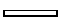
\includegraphics[height=20pt]{diagrams/PA_EOM1/PA_EOM1-figure22.pdf}}}.  Equation\ \eqref{eq:pa_1-body} generates the following expressions and corresponding diagrams, suppressing the state identifier $\mu$ for clarity,
\begin{align} \label{eq:pa_1-body-diagrams}
  \omega\rop{a}{} &= \sum\limits_{c}\xint{a}{c}\rop{c}{} + \sum\limits_{kc}\xint{k}{c}\rop{ac}{k} + \frac{1}{2}\sum\limits_{kcd}\xint{ak}{cd}\rop{cd}{k} \notag \\
  \diagram{PA_EOM1/PA_EOM1-figure0} &= \diagram{PA_EOM1/PA_EOM1-figure1} + \diagram{PA_EOM1/PA_EOM1-figure2} + \diagram{PA_EOM1/PA_EOM1-figure3}.
\end{align}
The corresponding expressions and diagrams for Eq.\ \eqref{eq:pa_2-body} are,
\begin{align} \label{eq:pa_2-body-diagrams}
  \omega\rop{ab}{i} &= \sum\limits_{c}\xint{ab}{ci}\rop{c}{} + \Perm{ab}\sum\limits_{c}\xint{b}{c}\rop{ac}{i} - \sum\limits_{k}\xint{k}{i}\rop{ab}{k} + \frac{1}{2}\sum\limits_{cd}\xint{ab}{cd}\rop{cd}{i} \notag \\
  &-\Perm{ab}\sum\limits_{kc}\xint{ak}{ci}\rop{cb}{k} - \frac{1}{2}\sum\limits_{klcd}\vint{kl}{cd}\amp{ab}{ki}\rop{cd}{l} \notag \\
  \diagram{PA_EOM1/PA_EOM1-figure4} &= \diagram{PA_EOM1/PA_EOM1-figure5} + \diagram{PA_EOM1/PA_EOM1-figure6} + \diagram{PA_EOM1/PA_EOM1-figure7} + \diagram{PA_EOM1/PA_EOM1-figure8} \notag \\
  &+ \diagram{PA_EOM1/PA_EOM1-figure9} + \diagram{PA_EOM1/PA_EOM1-figure10}.
\end{align}

The vector-matrix product for the left eigenvalue problem of the PA-EOM(2) method also consists of two components achieved in a similar fashion by right-multiplying Eq.\ \eqref{eq:eom_dual1} with the particle-attached ket states, $\statebra{a}{}$ and $\statebra{ab}{i}$, respectively, which has the effect of projecting out the corresponding components $\lint{\mu}{}{}$,
\begin{gather}
  \label{eq:pa_l_1-body}
  \refbra\Lop_{\mu}\EHamN\stateket{a}{} = \Ecorr_{\mu}\lint{\mu}{}{a}, \\
  \label{eq:pa_l_2-body}
  \refbra\Lop_{\mu}\EHamN\stateket{ab}{i} = \Ecorr_{\mu}\lint{\mu}{i}{ab}.
\end{gather}
Because Eqns.\ \eqref{eq:pa_l_1-body} and \eqref{eq:pa_l_2-body} do not use commutators between $\EHamN$ and $\Lop_{\mu}$, the diagrams which describe these equations include disconnected diagrams and corresponding expressions with matrix elements that share no indices.  For these diagrams, the left EOM de-excitation operators are depicted by the vertex type \raisebox{-8pt}{\mbox{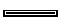
\includegraphics[height=20pt]{diagrams/PA_EOM1/PA_EOM1-figure23.pdf}}}.  Equation\ \eqref{eq:pa_l_1-body} generates the following expressions and diagrams, again supressing the state identifier $\mu$,
\begin{align} \label{eq:pa_l_1-body-diagrams}
  E\lop{}{a} &= \sum\limits_{c}\lop{}{c}\xint{c}{a} + \frac{1}{2}\sum\limits_{kcd}\lop{k}{cd}\xint{cd}{ak} \notag \\
  \diagram{PA_EOM1/PA_EOM1-figure11} &= \diagram{PA_EOM1/PA_EOM1-figure12} + \diagram{PA_EOM1/PA_EOM1-figure13}.
\end{align}
The corresponding expressions and diagrams for Eq.\ \eqref{eq:pa_l_2-body} are,
\begin{align} \label{eq:pa_l_2-body-diagrams}
  E\lop{i}{ab} &= \Perm{ab}\lop{}{a}\xint{i}{b} + \sum\limits_{c}\lop{}{c}\xint{ci}{ab} - \sum\limits_{k}\lop{k}{ab}\xint{i}{k} + \Perm{ab}\sum\limits_{c}\lop{i}{ac}\xint{c}{b} \notag \\
  &+ \frac{1}{2}\sum\limits_{cd}\lop{i}{cd}\xint{cd}{ab} - \Perm{ab}\sum\limits_{kc}\lop{k}{cb}\xint{ci}{ak} - \frac{1}{2}\sum\limits_{klcd}\lop{l}{cd}\vint{ki}{ab}\amp{cd}{kl} \notag \\
  \diagram{PA_EOM1/PA_EOM1-figure14} &= \diagram{PA_EOM1/PA_EOM1-figure15} + \diagram{PA_EOM1/PA_EOM1-figure16} + \diagram{PA_EOM1/PA_EOM1-figure17} + \diagram{PA_EOM1/PA_EOM1-figure18} \notag \\
  &+ \diagram{PA_EOM1/PA_EOM1-figure19} + \diagram{PA_EOM1/PA_EOM1-figure20} + \diagram{PA_EOM1/PA_EOM1-figure21}.
\end{align}

The particle-removed equations are generated in exactly the same way.  The matrix-vector product for the right eigenvalue problem of the PR-EOM(2) method consists of two components corresponding to the particle-removed bra states, $\statebra{}{i}$ and $\statebra{a}{ij}$, respectively,
\begin{gather}
  \label{eq:pr_1-body}
  \statebra{}{i}\left( \EHamN\Rop_{\mu} \right)_{\mathrm{c}}\refket = \omega_{\mu}\rint{\mu}{}{i}, \\
  \label{eq:pr_2-body}
  \statebra{a}{ij}\left( \EHamN\Rop_{\mu} \right)_{\mathrm{c}}\refket = \omega_{\mu}\rint{\mu}{a}{ij}.
\end{gather}
Equation\ \eqref{eq:pr_1-body} generates the following expressions and diagrams,
\begin{align} \label{eq:pr_1-body-diagrams}
  \omega\rop{}{i} &= -\sum\limits_{k}\xint{k}{i}\rop{}{k} + \sum\limits_{kc}\xint{k}{c}\rop{c}{ik} - \frac{1}{2}\sum\limits_{klc}\xint{kl}{ic}\rop{c}{kl} \notag \\
  \diagram{PR_EOM1/PR_EOM1-figure0} &= \diagram{PR_EOM1/PR_EOM1-figure1} + \diagram{PR_EOM1/PR_EOM1-figure2} + \diagram{PR_EOM1/PR_EOM1-figure3}.
\end{align}
The corresponding expressions and diagrams for Eq.\ \eqref{eq:pr_2-body} are,
\begin{align} \label{eq:pr_2-body-diagrams}
  \omega_{k}\rop{a}{ij} &= -\sum\limits_{k}\xint{ka}{ij}\rop{}{k} - \Perm{ij}\sum\limits_{k}\xint{k}{j}\rop{a}{ik} + \sum\limits_{c}\xint{a}{c}\rop{c}{ij} + \frac{1}{2}\sum\limits_{kl}\xint{kl}{ij}\rop{a}{kl} \notag \\
  &-\Perm{ij}\sum\limits_{kc}\xint{ak}{ci}\rop{c}{kj} - \frac{1}{2}\sum\limits_{klcd}\vint{kl}{cd}\amp{ca}{ij}\rop{d}{kl} \notag \\
  \diagram{PR_EOM1/PR_EOM1-figure4} &= \diagram{PR_EOM1/PR_EOM1-figure5} + \diagram{PR_EOM1/PR_EOM1-figure6} + \diagram{PR_EOM1/PR_EOM1-figure7} + \diagram{PR_EOM1/PR_EOM1-figure8} \notag \\
  &+ \diagram{PR_EOM1/PR_EOM1-figure9} + \diagram{PR_EOM1/PR_EOM1-figure10}.
\end{align}

Finally, the vector-matrix product for the left eigenvalue problem of the PA-EOM(2) method consists of two components which correspond with the particle-removed ket states, $\statebra{}{i}$ and $\statebra{a}{ij}$, respectively,
\begin{gather}
  \label{eq:pr_l_1-body}
  \refbra\Lop_{\mu}\EHamN\stateket{}{i} = \Ecorr_{\mu}\lint{\mu}{i}{}, \\
  \label{eq:pr_l_2-body}
  \refbra\Lop_{\mu}\EHamN\stateket{a}{ij} = \Ecorr_{\mu}\lint{\mu}{ij}{a}.
\end{gather}
Again, Eqns.\ \eqref{eq:pr_l_1-body} and \eqref{eq:pr_l_2-body} do not remove disconnected diagrams with commutator between $\EHamN$ and $\Lop_{\mu}$.  Equation\ \eqref{eq:pr_l_1-body} generates the following expressions and diagrams,
\begin{align} \label{eq:pr_l_1-body-diagrams}
  E\lop{i}{} &= -\sum\limits_{k}\lop{k}{}\xint{i}{k} - \frac{1}{2}\sum\limits_{klc}\lop{kl}{c}\xint{ic}{kl} \notag \\
  \diagram{PR_EOM1/PR_EOM1-figure11} &= \diagram{PR_EOM1/PR_EOM1-figure12} + \diagram{PR_EOM1/PR_EOM1-figure13}.
\end{align}
The corresponding expressions and diagrams for Eq.\ \eqref{eq:pr_l_2-body} are,
\begin{align} \label{eq:pr_l_2-body-diagrams}
  E_{k}\lop{ij}{a} &= \Perm{ij}\lop{i}{}\xint{j}{a} - \sum\limits_{k}\lop{k}{}\xint{ij}{ka} + \sum\limits_{c}\lop{ij}{c}\xint{c}{a} - \Perm{ij}\sum\limits_{k}\lop{ik}{a}\xint{j}{k} \notag \\
  &+ \frac{1}{2}\sum\limits_{cd}\lop{kl}{a}\xint{ij}{kl} - \Perm{ij}\sum\limits_{kc}\lop{kj}{c}\xint{ci}{ak} - \frac{1}{2}\sum\limits_{klcd}\lop{kl}{d}\vint{ij}{ca}\amp{cd}{kl} \notag \\
  \diagram{PR_EOM1/PR_EOM1-figure14} &= \diagram{PR_EOM1/PR_EOM1-figure15} + \diagram{PR_EOM1/PR_EOM1-figure16} + \diagram{PR_EOM1/PR_EOM1-figure17} + \diagram{PR_EOM1/PR_EOM1-figure18} \notag \\
  &+ \diagram{PR_EOM1/PR_EOM1-figure19} + \diagram{PR_EOM1/PR_EOM1-figure20} + \diagram{PR_EOM1/PR_EOM1-figure21}.
\end{align}

These expressions must be computed for every iteration of the Arnoldi algorithm and contain expensive sums that can benefit from the techniques of section \ref{section:solvingcc}.  The major difference in this case is that while the cluster operators and the Hamiltonian are scalar operators that define the conserve quantum numbers of a symmetry channel \ref{section:symmetry_channels}, the EOM operators 


\section{EOM-CC for 2D Quantum Dots} \label{section:eom_qd}

To examine some properties of the EOM-CC method, it's useful to focus on the results from the two-dimensional quantum dot.  This system, also known as an ``artificial atom'', consists of $A$ electrons confined within a 2D harmonic oscillator and subject to the inter-electron Coulomb force.  These nanoscale structures are easily tunable which makes them relevant for probing many different quantum phenomena in experiments and theoretical models \cite{REIMANN2002,ENGEL1993,BIRMAN20131}, and because the quantum dot shell structure is similar to those of atomic nuclei, they provide a useful system to quantify the impact of quantum effects at different levels of correlation \cite{TARUCHA1996}.

\subsection{Quantum Dot Formalism}

The circular quantum dot system is characterized by a harmonic-oscillator potential of the form $V(r) = m \omega^2r^2 / 2$, where $\omega$ is its angular frequency, $r$ is the radial distance from the center, and $m$ is the electron mass.  The single-particle states can be constructed as eigenfunctions of the 2D quantum harmonic oscillator,
\begin{equation} \label{eq:2d_ho}
  \left(\frac{-\hbar^{2}}{2m}\nabla^{2} + \frac{1}{2} m\omega^{2}r^{2}\right)\phi_{n m_{\ell} \sigma}(\mathbf{r}) = \epsilon_{n m_{\ell}}\phi_{n m_{\ell} \sigma}(\mathbf{r}).
\end{equation}
These states are characterized by a radial quantum number $n$, a spin quantum number $\sigma$, and because this systems conserves orbital angular momentum, a corresponding angular momentum projection number, $m_{\ell}$.  The energy of each single-particle state $\phi_{n m_{\ell} \sigma}(\mathbf{r})$, independent of the spin quantum projection, is given by,
\begin{align} \label{eq:energysingleparticlestate}
  \epsilon_{n m_{\ell}} \equiv (2 n + |m_\ell| + 1) \omega.
\end{align}
In addition to the spin projection $\sigma$, they are degenerate with respect to the \textit{shell index} $k$,
\begin{align} \label{eq:shell_index}
  k \equiv 2 n + |m_\ell|,
\end{align}
which labels each shell from zero with a total number of shells, $K$.  The shell structure is illustrated in Fig.\ \ref{fig:qd-shell-structure}.
\begin{figure}[h]
  \centering
  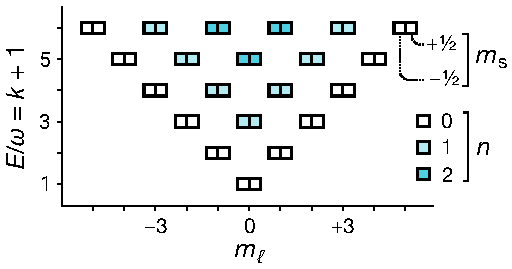
\includegraphics[width=0.75\linewidth]{EOM/fig-shell-structure-v2.pdf}
  \caption{The 42 lowest single-particle states (the first 5 shells) in the 2D harmonic oscillator basis.  Each box represents a single-particle state arranged by $m_\ell$, $m_{\mathrm{s}}$, and energy, and the up/down arrows indicate the spin of the states.  Within each column, the principal quantum number $n$ increases as one traverses upward.}
  \label{fig:qd-shell-structure}
\end{figure}

The specific form of these basis states can be solved with the cylindrically symmetric Fock--Darwin states $F_{n m_{\ell}}$, which conserve the orbital angular momentum projection $\hat{L}_{\mathrm{z}} \equiv -\mathrm{i} \frac{\partial}{\partial \varphi}$.  Apart from their spin component, the states are defined as \cite{LOHNE2010},
\begin{align}
  F_{n m_{\ell}}(\rho, \varphi) &\equiv \sqrt\omega R_{n |m_\ell|}(\sqrt \omega \rho) \times \frac{1}{\sqrt{2 \pi}} \mathrm{e}^{\mathrm{i} m_\ell \varphi} \label{eq:fockdarwin},\ \ \text{where} \\
  R_{n m}(\varrho) &\equiv \sqrt{\frac{2 \times n!}{(n + m)!}} \mathrm{e}^{-\varrho^2 / 2} \varrho^m L_n^{(m)}(\varrho^2) \notag
\end{align}
and $L_n^{(\alpha)}$ denotes the generalized Laguerre polynomial \cite{NIST:DLMF} of degree $n$ and parameter $\alpha$.

Like the homogeneous electron gas, (see section \ref{section:electrongas}), the electrons in the quantum dot interact with each other through the standard Coulomb interaction, $V\left( \mathbf{r}_{1}, \mathbf{r}_{2}\right) = 1/\lvert \mathbf{r}_{1} - \mathbf{r}_{2} \rvert$, which is expressed in atomic units where $m = c = e = (4\pi\epsilon_{0})^{-1} = 1$.  With the form of the single-particle wave functions, the second-quantized form of the two-body interaction can be analytically calculated,
\begin{equation} \label{eq:coloumb_integral}
  \Hint{2}{pq}{rs} \equiv \int d\mathbf{r}_{1} d\mathbf{r}_{2}\ \phi^{*}_{p}(\mathbf{r_{1}})\phi^{*}_{q}(\mathbf{r}_{2}) \frac{1}{\lvert \mathbf{r}_{1} - \mathbf{r}_{2} \rvert} \left[\phi_{r}(\mathbf{r}_{1})\phi_{s}(\mathbf{r}_{2}) - \phi_{s}(\mathbf{r}_{1})\phi_{r}(\mathbf{r}_{2})\right],
\end{equation}
where $\phi_{p}(\mathbf{r})$ is shorthand for $\phi_{n_{p} m_{\ell_{p}}\sigma_{p}}(\mathbf{r})$.

With these ingredients in hand, the ground state energy, as well as particle-attached and particle-removed energies, can be calculated for different values of the oscillator frequency, $\omega$, and the number of shells, $K$.

\subsection{Quantum Dot Results}

Here, CC results are shown along with results from the in-medium similarity renormalization group (IM-SRG) method, and quasi-degenerate perturbation theory (QDPT) \cite{LINDGREN1974}.  As for all calculations in this work, each method applies a Hartree-Fock transformation of the basis states from Eq.\ \eqref{eq:2d_ho} before employing the primary many-body method.  Before analyzing the EOM results, the ground state energies calculated using CCSD and IM-SRG(2) are shown in Fig. \ref{fig:QDground}.  Also included are results from M\o ller--Plesset perturbation theory to second order (MP2), DMC \cite{HOGBERGET2013}, and full CI \cite{OLSEN2013} for comparison where available.

\begin{figure}[h]
  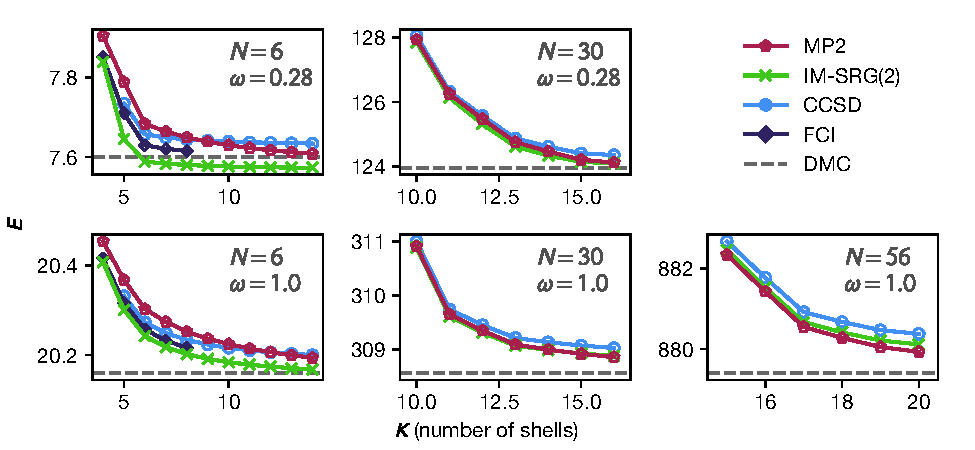
\includegraphics[width=\linewidth]{EOM/fig-gs2.pdf}
  \caption{Ground state energy (in Hartrees) of quantum dots with $N$ particles and an oscillator frequency of $\omega$ calculated with several different methods.}
  \label{fig:QDground}
\end{figure}

With respect to the number of shells, both IM-SRG(2) and CCSD appear to converge slightly faster than second order perturbation theory (MP2), mainly due to the presence of higher order corrections in IM-SRG(2) and CCSD.  However, the main conclusion that can be reached from Fig. \ref{fig:QDground} is the overall convergence between vastly different methods, a hallmark of properly-treated \emph{ab initio} methods.

Additionally, the results for addition and removal energy calculations are summarized in Fig.\ \ref{fig:QDadd} and Fig.\ \ref{fig:QDrm} respectively.  Not only do these results reaffirm the validity of the CCSD method amongst other \emph{ab initio} methods, they also provide benchmark calculations for the following CC-EOM calculations of open-shell finite nuclei.

\begin{figure}
  \centering
  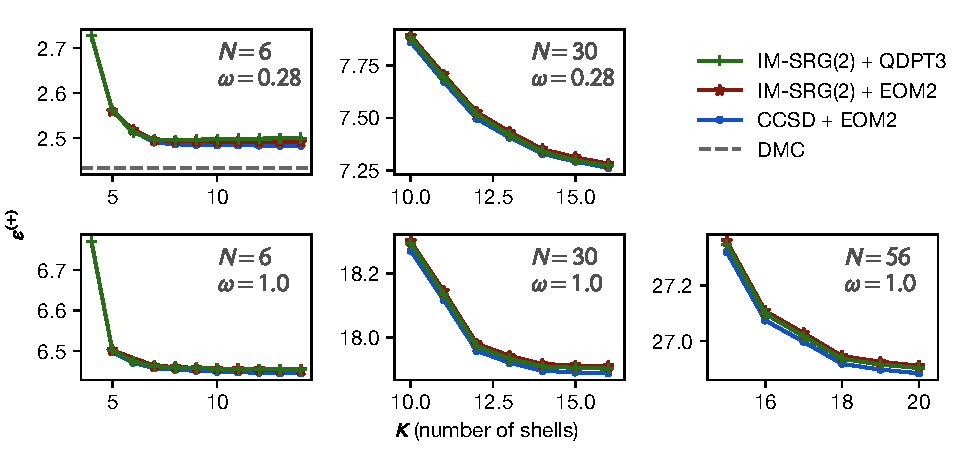
\includegraphics[width=\textwidth]{EOM/fig-add2.pdf}
  \caption{Particle-attached energy (in Hartrees) of quantum dots with $N$ particles and an oscillator frequency of $\omega$ calculated with several different methods.}
  \label{fig:QDadd}
\end{figure}

\begin{figure}
  \centering
  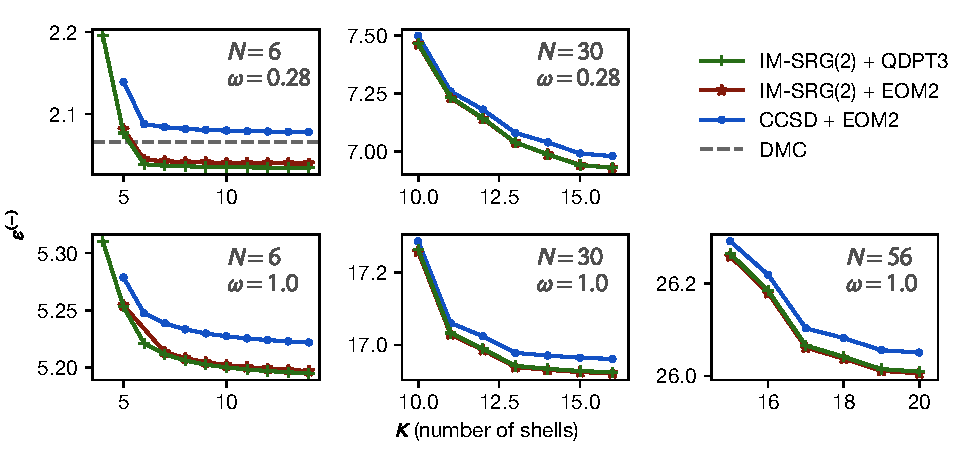
\includegraphics[width=\textwidth]{EOM/fig-rm2.pdf}
  \caption{Particle-removed energy (in Hartrees) of quantum dots with $N$ particles and an oscillator frequency of $\omega$ calculated with several different methods.}
  \label{fig:QDrm}
\end{figure}


\section{Quality of EOM Solutions} \label{section:eom_quality}

Applying the CC similarity transformation to the Hamiltonian implicitly re-sums contributions from higher order excitations beyond the EOM(2)-CC truncation ($\ph{3}{2}$, $\ph{4}{3}$, \ldots for PA-EOM and $\ph{2}{3}$, $\ph{3}{4}$, \ldots for PR-EOM) into the lower-order excitations which comprise the EOM(2)-CC operators ($\ph{1}{0}$, $\ph{2}{1}$, \ldots for PA-EOM and $\ph{0}{1}$, $\ph{1}{2}$, \ldots for PR-EOM).  This means that EOM states are weighted towards few-body excitations when compared to the corresponding state calculated with the CI method and the bare Hamiltonian.

Despite this improvement on the corresponding CI method, the EOM(2) truncation of Eqs.\ \eqref{eq:pa-eom2} and \eqref{eq:pr-eom2} is not guaranteed to capture the primary components of certain collective states.  Therefore, the quality of the solution can be judged by the measuring the amount of overlap between the EOM solution and $\ph{1}{0}$ states for PA-EOM or $\ph{0}{1}$ states for PR-EOM.  This overlap can be computed with partial norms,
\begin{align}
  \label{eq:partial_norms_p}
  n_{\text{1-particle}} &= \sqrt{\sum_{a} \statebra{a}{}\Rop_{\mu}\refket\refbra\Lop_{\mu}\stateket{a}{} } = \sqrt{\sum_{a} \lvert \rint{}{a}{}\lint{}{}{a} \rvert },\\
  \label{eq:partial_norms_h}
  n_{\text{1-hole}} &= \sqrt{\sum_{i} \statebra{}{i}\Rop_{\mu}\refket\refbra\Lop_{\mu}\stateket{}{i} } = \sqrt{\sum_{i} \lvert \rint{}{}{i}\lint{}{i}{} \rvert }.
\end{align}
If the single-particle overlap is small, the state is dominated by higher-order excitations and requires a less-restricted truncation to describe, which can be accomplished directly or perturbatively \cite{PARZUCHOWSKI2017044304,MORRIS2017}.  On the other hand, large single-particle partial norms indicate that the EOM truncation is reasonable for the relevant state.

Figure \ref{fig:EOM-Quality} shows this relationship using the difference between EOM-CC and full CI energies for quantum dot particle-attached and particle-removed states, $\mathrm{\Delta E/E}$, as function of the single-particle overlap.  The energy difference with the exact FCI result grows as the single-particle character of the wave function shrinks.  Therefore, care should be taken when encountering unphysical states with a small single-particle overlap.
\begin{figure}[h]
  \centering
  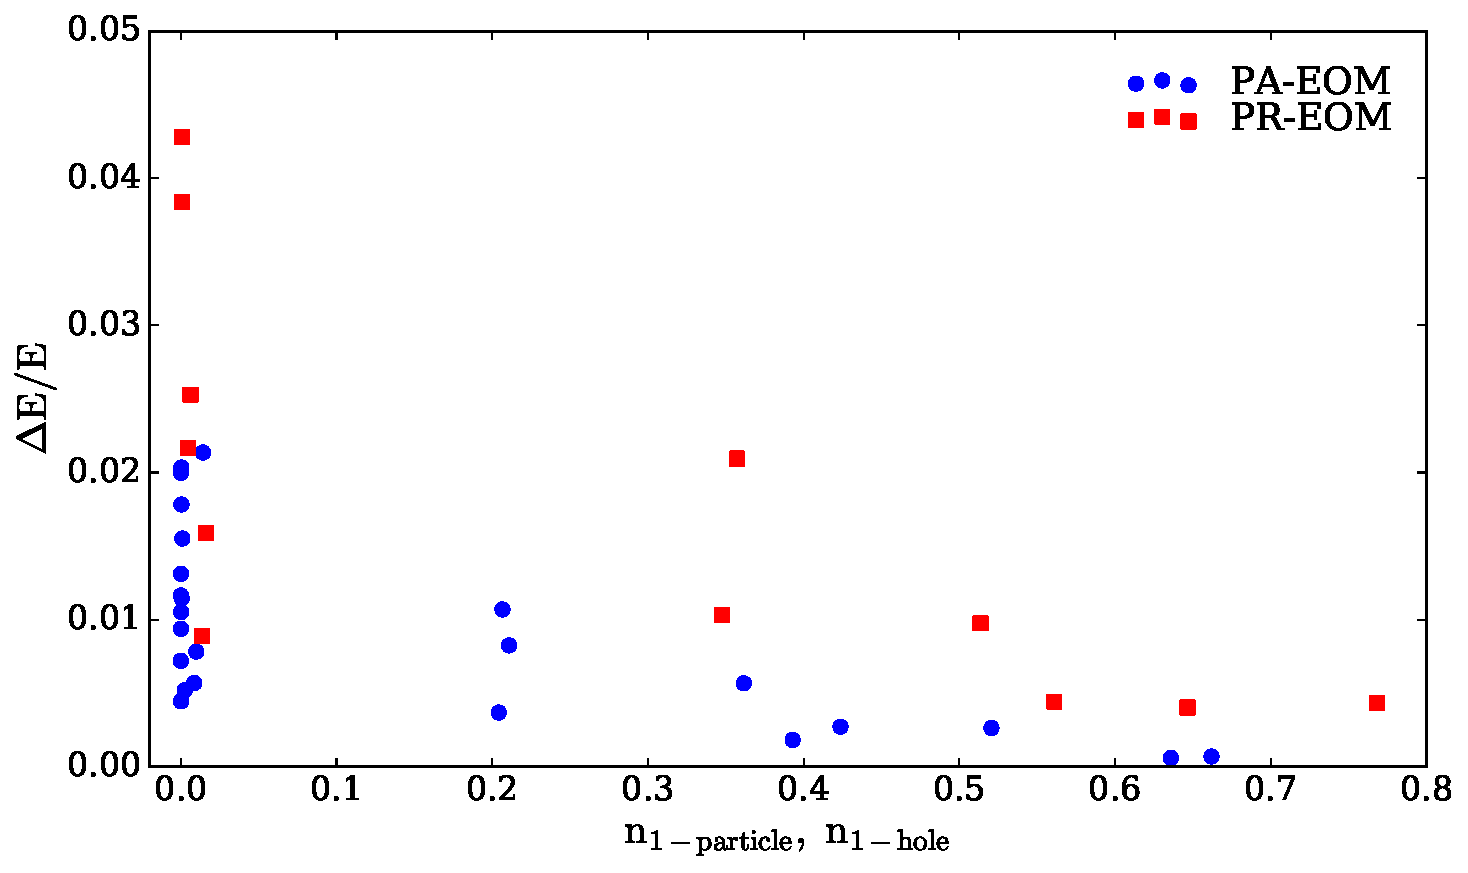
\includegraphics[width=0.9\linewidth]{EOM/QD_EOM.pdf}
  \caption{Energy difference of particle-attached and particle-removed states between the EOM-CC method and the exact FCI method for a quantum dot with various parameters plotted against the single-particle overlap of the FCI state, $n_{\text{1-particle}}$ or $n_{\text{1-hol}}$, see Eqs.\ \eqref{eq:partial_norms_p} and \eqref{eq:partial_norms_h}.  The strong correlation shows that the quality of EOM states can be judged by this metric.}
  \label{fig:EOM-Quality}
\end{figure}


\section{EOM-CC for Finite Nuclei} \label{section:eom_nuclei}

Like its ground-state counterpart, the EOM extension to coupled cluster theory was first applied to nuclear systems \cite{EMRICH1981379,EMRICH1981397,EMRICH1981439}.  However the progress was again halted by the non-perturbative nucleon-nucleon interaction, so again it quickly gained prominance in quantum chemistry \cite{STANTON1993,SHAVITT2009}.  Since the intruduction of SRG-softened chiral interaction, the EOM-CC method has been established as a powerful and reliable method for reaching open-shell systems and excited states \cite{WLOCH2005212501,GOUR2006024310,JANSEN2013,HAGEN2012,EKSTROM2015}.  This section shows results for the PA-EOM-CC and PR-EOM-CC methods calculated with the NN+3N(400) interaction, SRG softened with $\lambda_{\mathrm{SRG}}=2.0\ \mathrm{fm}^{-1}$.  The initial closed-shell calculations were performed for $^{16}$O and $^{22}$O.

The ground-state energies for particle-attached nuclei are shown in Fig. \ref{fig:PA-Nuclei}.  Unlike the ground states for closed-shell nuclei, which is uniquely determined, the particle-attached ground state must be identified as the state corresponding to the lowest eigenvalue of the converged solution.  All the results are in close agreement with the experimental values while the subshell nuclei, $^{23}$O and $^{23}$F, are slightly underbound like their closed-shell counterpart, $^{16}$O (see Fig.\ \ref{fig:Ground_State2}).
\begin{figure}[h]
  \centering
  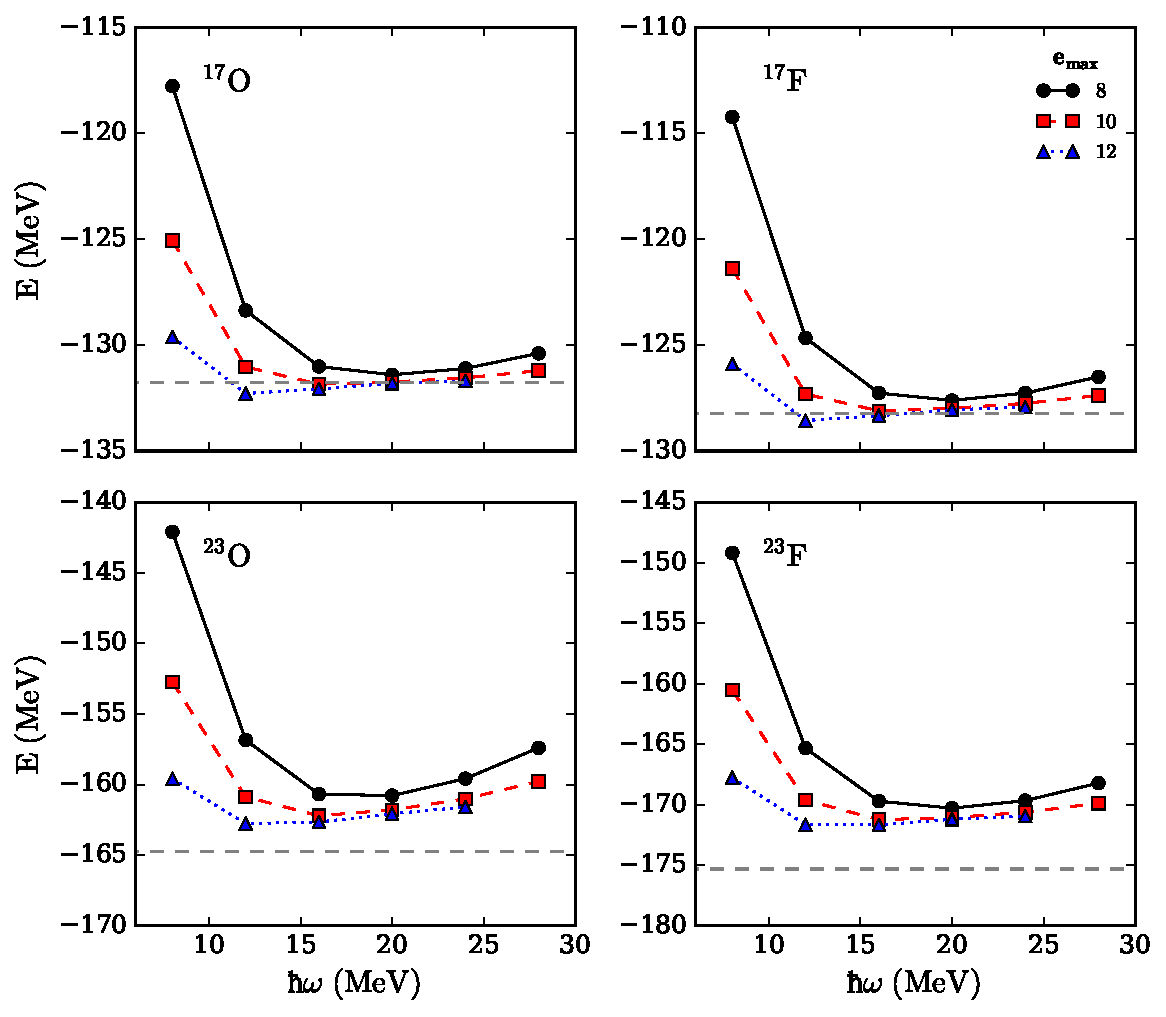
\includegraphics[width=\linewidth]{EOM/PA-EOM.pdf}
  \caption{Ground-state energies for the particle-attached nuclei $^{17}$O, $^{17}$F, $^{23}$O, and $^{23}$F as a function of the harmonic oscillator energy $\hbar\omega$ with the NN+3N(400) interaction, SRG softened with $\lambda_{\mathrm{SRG}}=2\mathrm{fm}^{-1}$.  The energies are plotted for $e_\mathrm{max}=8,10,12$, showing the convergence as the model space increases.  The grey dashed line is the experimental binding energy.}
  \label{fig:PA-Nuclei}
\end{figure}

The ground-state energies for particle-removed nuclei are shown in Fig. \ref{fig:PR-Nuclei}.  These results follow the same pattern as the particle-attached states, converging to within $\sim 1\%$ at $e_{\mathrm{max}}=12$ and overbinding for EOM states constructed from the $^{22}$O ground state.
\begin{figure}[h]
  \centering
  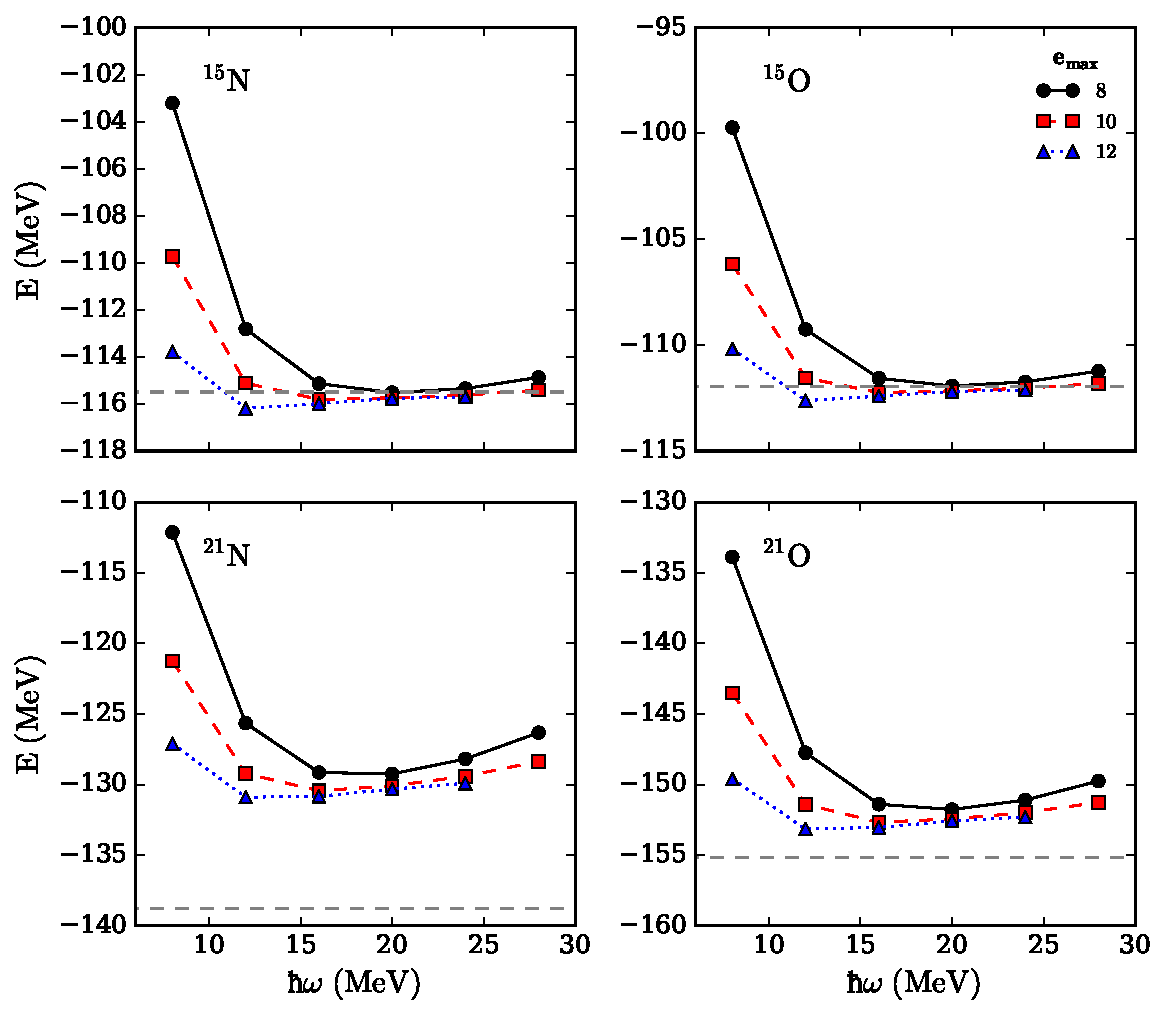
\includegraphics[width=\linewidth]{EOM/PR-EOM.pdf}
  \caption{Ground-state energies for the particle-removed nuclei $^{15}$N, $^{15}$O, $^{21}$N, and $^{21}$O as a function of the harmonic oscillator energy $\hbar\omega$ with the NN+3N(400)-induced interaction, SRG softened with $\lambda_{\mathrm{SRG}}=2\mathrm{fm}^{-1}$.  The energies are plotted for $e_\mathrm{max}=8,10,12$, showing the convergence as the model space increases.  The grey dashed line is the experimental binding energy.}
  \label{fig:PR-Nuclei}
\end{figure}

The problem of center-of-mass contamination discussed in section \ref{section:CoM} extends to the EOM states as well.  To ensure that the EOM wavefunction has been sufficiently factorized from the COM wave function, an equivalent diagnostic to Fig. \ref{fig:CoM_Ground_State} can be performed.  First, the ground-state COM energy is computed using Eq.\ \eqref{eq:com_energy} and the corresponding COM oscillator strength is obtained from Eq.\ \eqref{eq:com_hw}.  By using $A+1$ particles for PA-EOM and $A-1$ particles for PR-EOM in the intrinsic Hamiltonian, Eq.\ \eqref{eq:intrinsic_hamiltonian}, the $A$-body problem is not properly treated.  However, the approximate COM factorization for the $A+1$ and $A-1$ systems, according to Eq. \eqref{eq:com_factorize}, is reached when the COM energy vanishes at this new oscillator strength.  The results from the COM diagnostic on the PA-EOM and PR-EOM states is shown in Fig. \ref{fig:EOM_COM}.
\begin{figure}[h]
  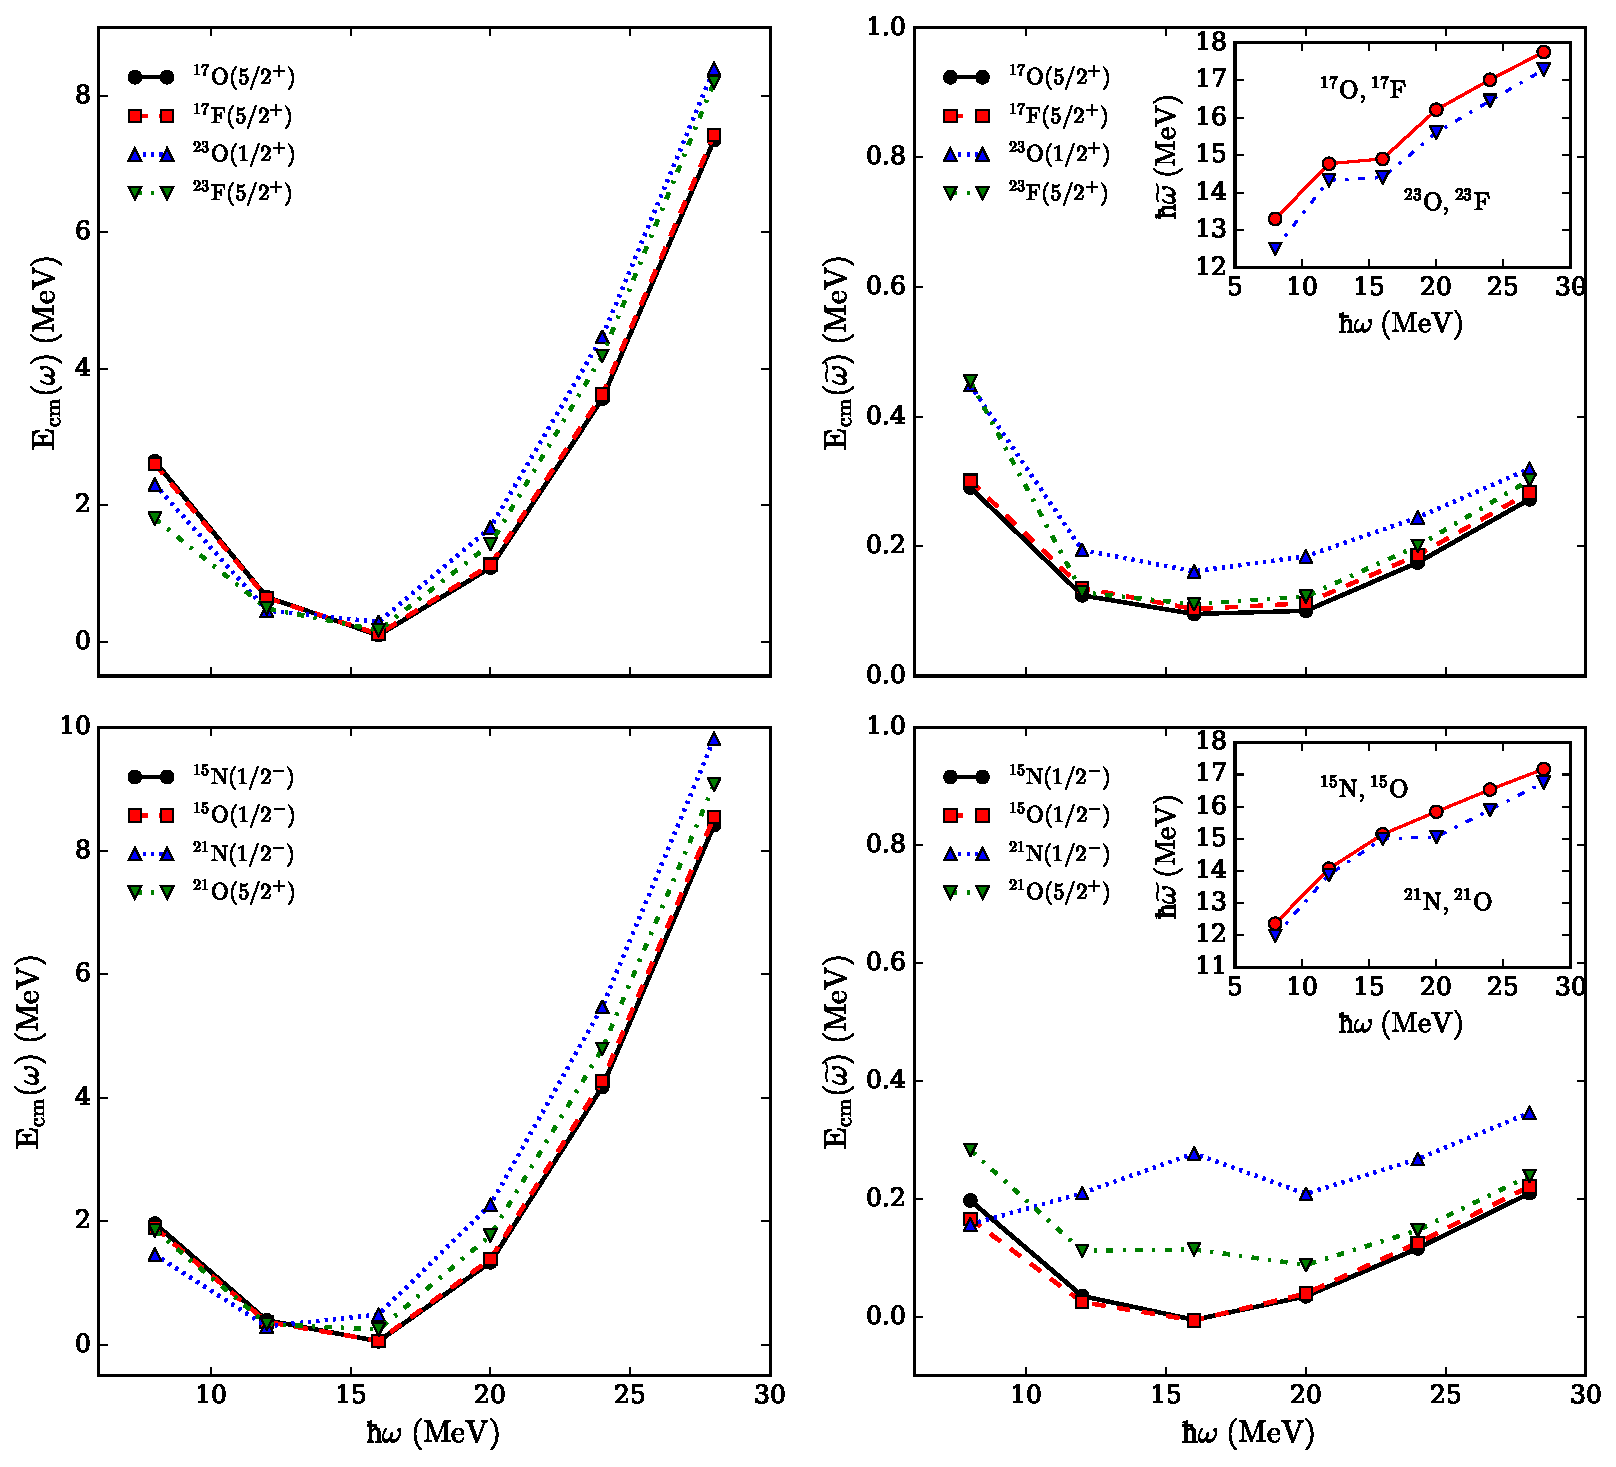
\includegraphics[width=\linewidth]{EOM/EOM-CoM.pdf}
  \caption{Ground-state COM energies, Eq.\ \eqref{eq:com_hamiltonian}, for open-shell nuclei at varies harmonic oscillator frequencies with the NN+3N(400)-induced interaction with $\lambda_{\mathrm{SRG}}=2.0\ \mathrm{fm}^{-1}$ at $e_{\mathrm{max}}=12$.  The top row shows the results for the particle-attached nuclei ${}^{17}$O, ${}^{17}$F, ${}^{23}$O, and ${}^{23}$F, and the bottom row shows the results for the particle-removed nuclei ${}^{15}$N, ${}^{15}$O, ${}^{21}$N, and ${}^{21}$O.  The right column shows that the COM wave function practically vanishes according to Eq.\ \eqref{eq:com_factorize}.}
  \label{fig:EOM_COM}
\end{figure}

With the underlying COM oscillator strengths determined from Fig. \ref{fig:EOM_COM}, the excitation spectra of the corresponding open-shell nuclei can be treated with the Lawson-Gloeckner method \cite{GLOECKNER1974313} by artificially raising COM-coupled, spurious states out of the range of interest by adding the COM Hamiltonian to the intrinsic Hamiltonian, Eq.\ \eqref{eq:lawson-term}.  The EOM low-lying excited states of $^{17}$O and $^{17}$F are shown in Fig. \ref{fig:O17F17_spectra} with and without the Lawson-Gloeckner term.  When the term is added, the spurious negative-partiy states are removed from the lower portion of the spectra.  The non-spurious states, $1/2^{+}$ and $3/2^{+}$, are not removed but do increase slightly due to the imperfect COM factorization.

\begin{figure}[h]
  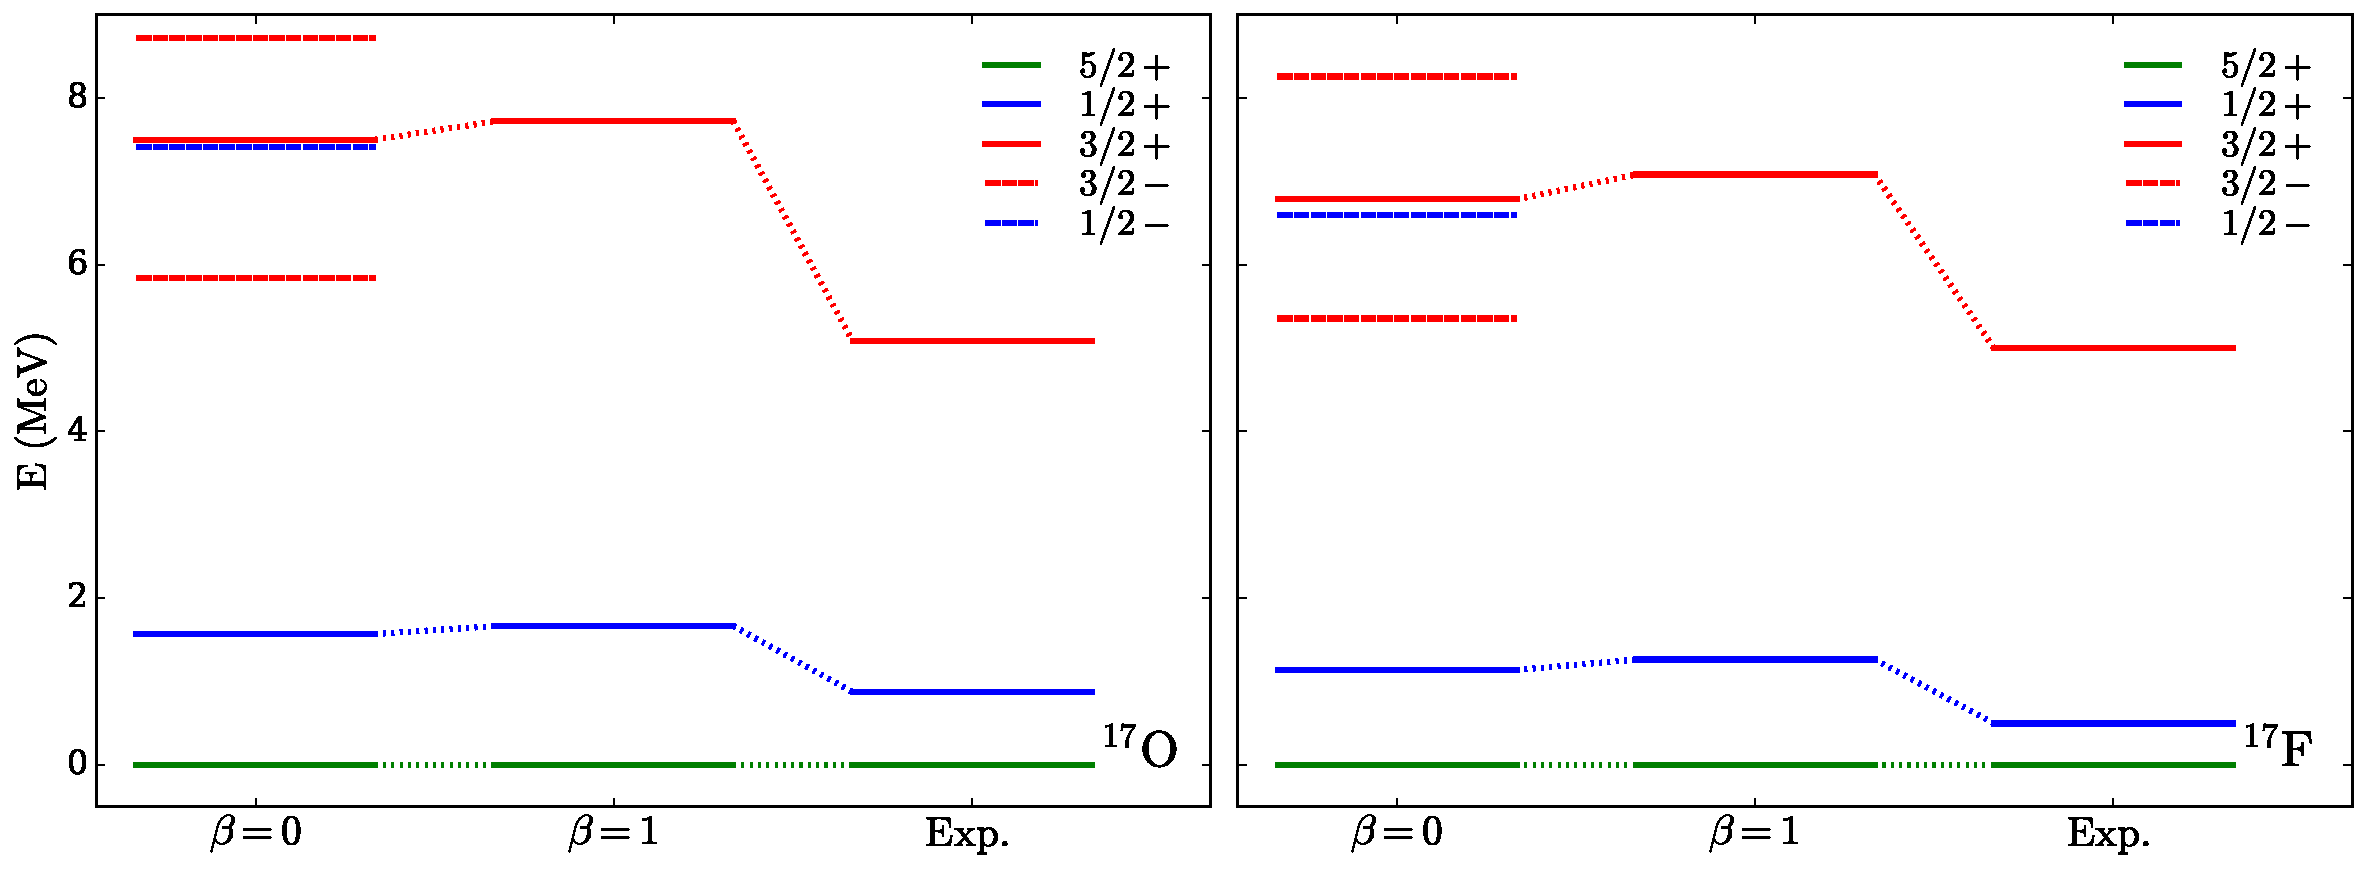
\includegraphics[width=\linewidth]{EOM/O17_F17_EOM_2.pdf}
  \caption{Low-lying PA-EOM states for $^{17}$O and $^{17}$F with and without a Lawson-Gloeckner term, along with the experimentally determined spectra.  The negative-partity states are COM contaminants and are removed by artificially raising the COM excitation energy with the parameter $\beta$ according to Eq.\ \eqref{eq:lawson-term}.}
  \label{fig:O17F17_spectra}
\end{figure}

\begin{figure}[h]
  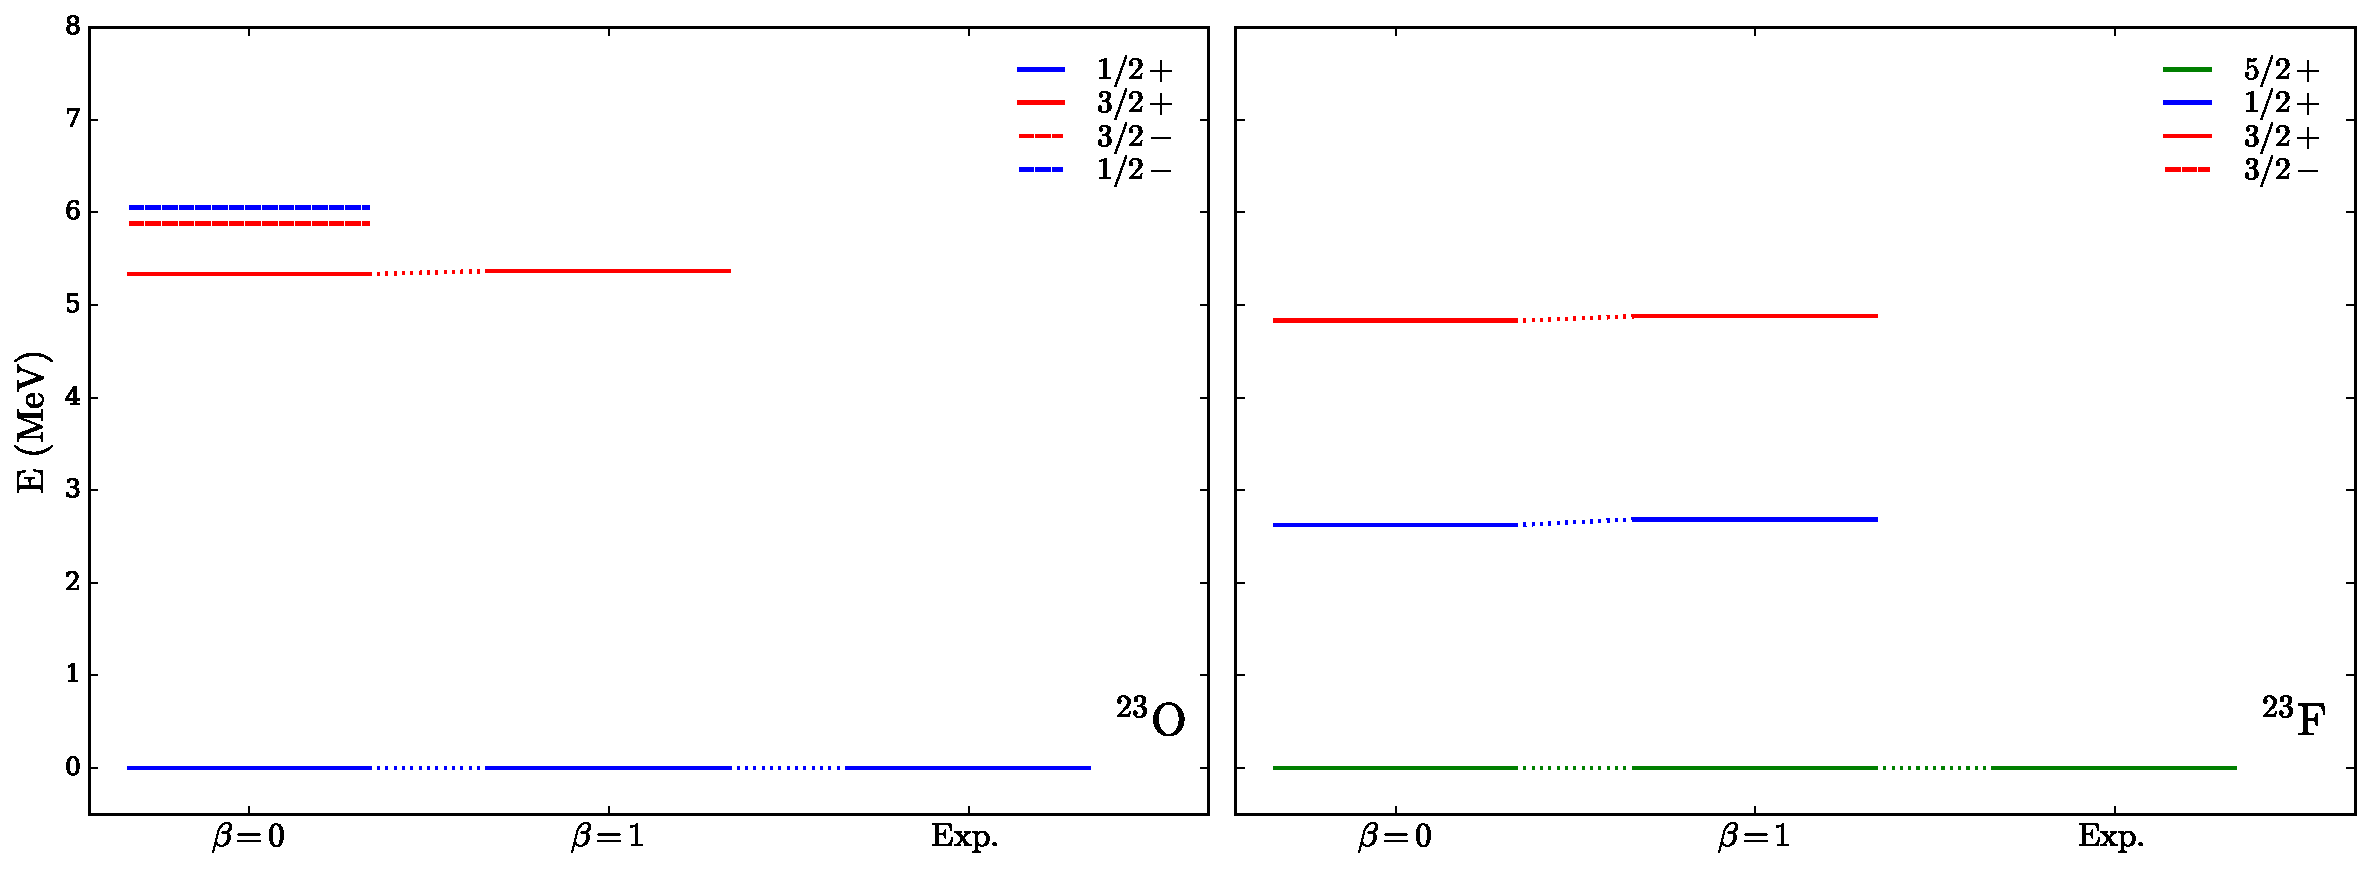
\includegraphics[width=\linewidth]{EOM/O23_F23_EOM_2.pdf}
  \caption{Low-lying PA-EOM states for $^{23}$O and $^{23}$F with and without a Lawson-Gloeckner term.  The negative-partiy states in $^{17}$O are COM contaminants and are removed by artificially raising the COM excitation energy with the Lawson-Gloeckner method, Eq.\ \eqref{eq:lawson-term}.  The excited states of these nuclei have not been experimentally detemined.}
  \label{fig:O23F23_spectra}
\end{figure}

\begin{figure}[h]
  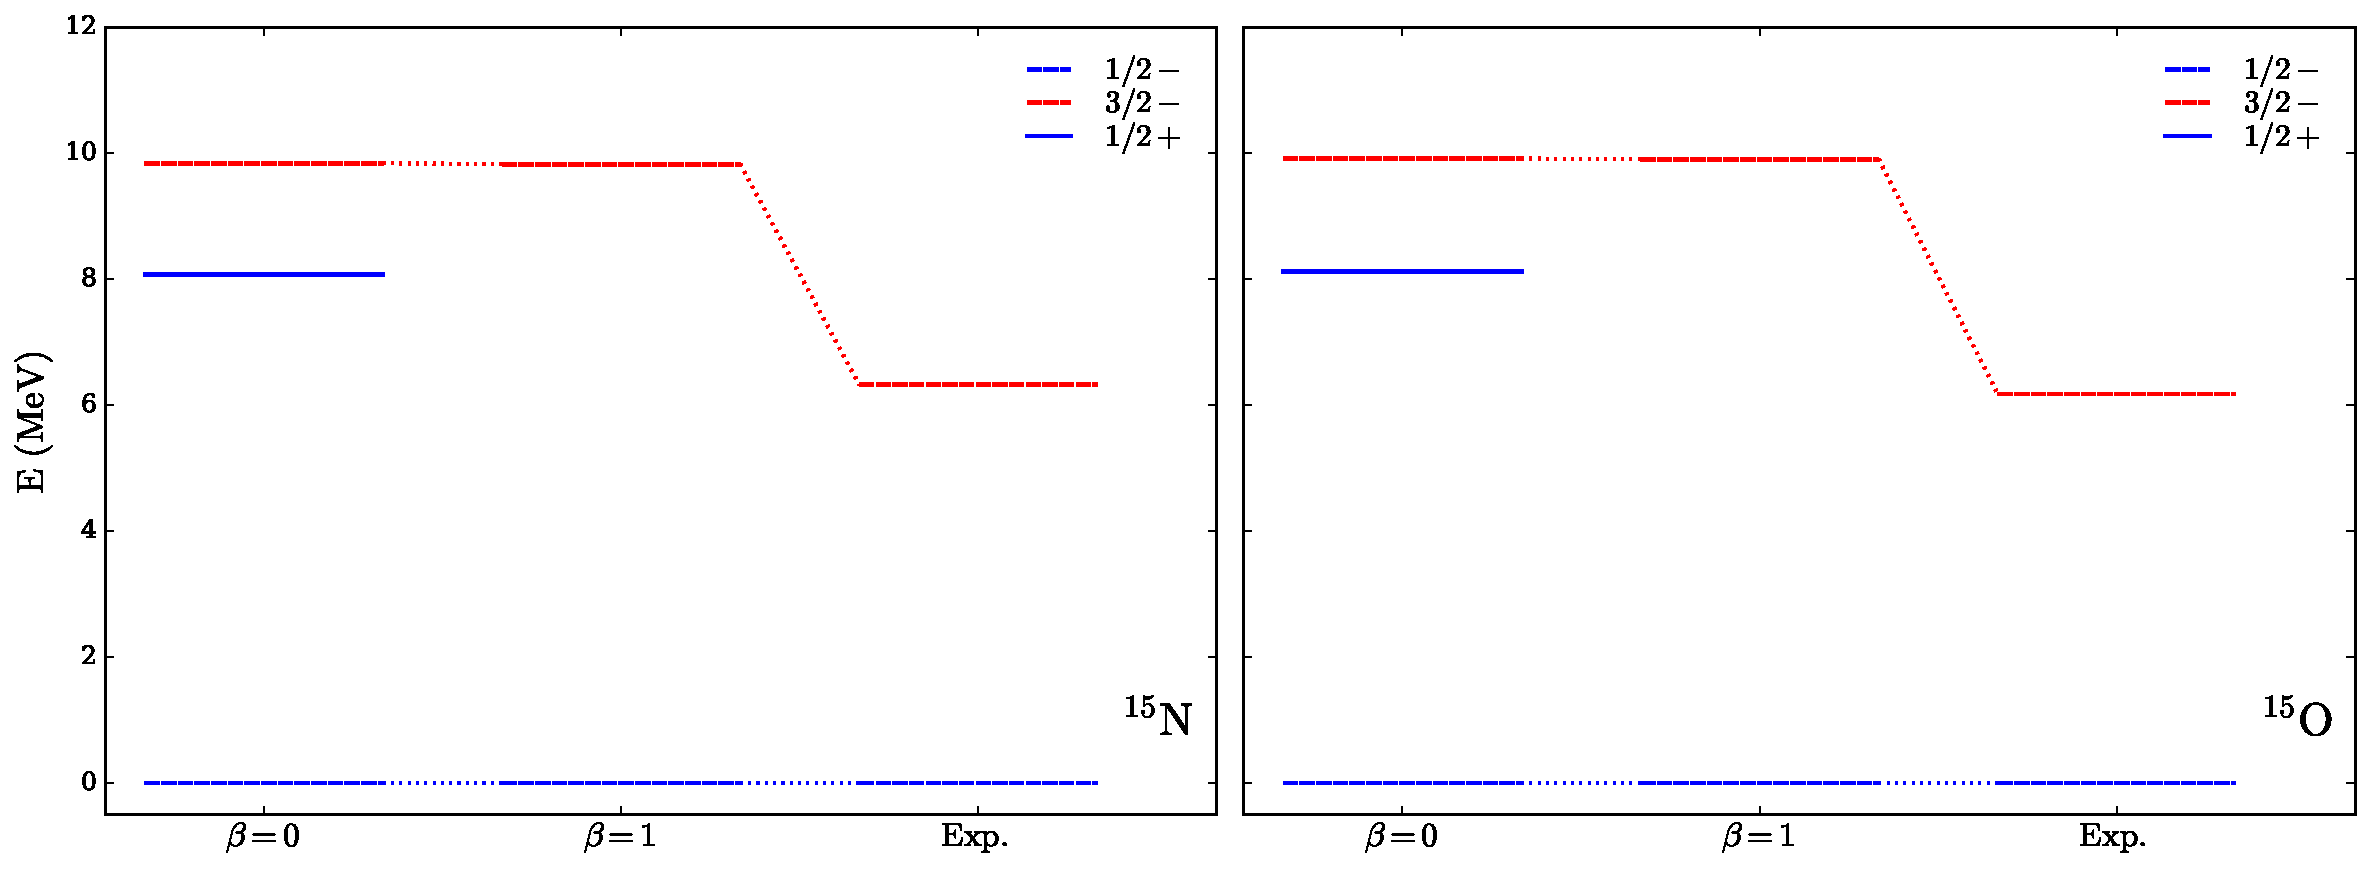
\includegraphics[width=\linewidth]{EOM/N15_O15_EOM_2.pdf}
  \caption{Low-lying PR-EOM states for $^{15}$N and $^{15}$O with and without a lawson-gloeckner term, and the experimentally determined spectra.  The $1/2^{+}$ state is a COM contaminant and is removed by artificially raising the COM excitation energy with the parameter $\beta$ according to Eq.\ \eqref{eq:lawson-term}.}
  \label{fig:N15O15_spectra}
\end{figure}

\begin{figure}[h]
  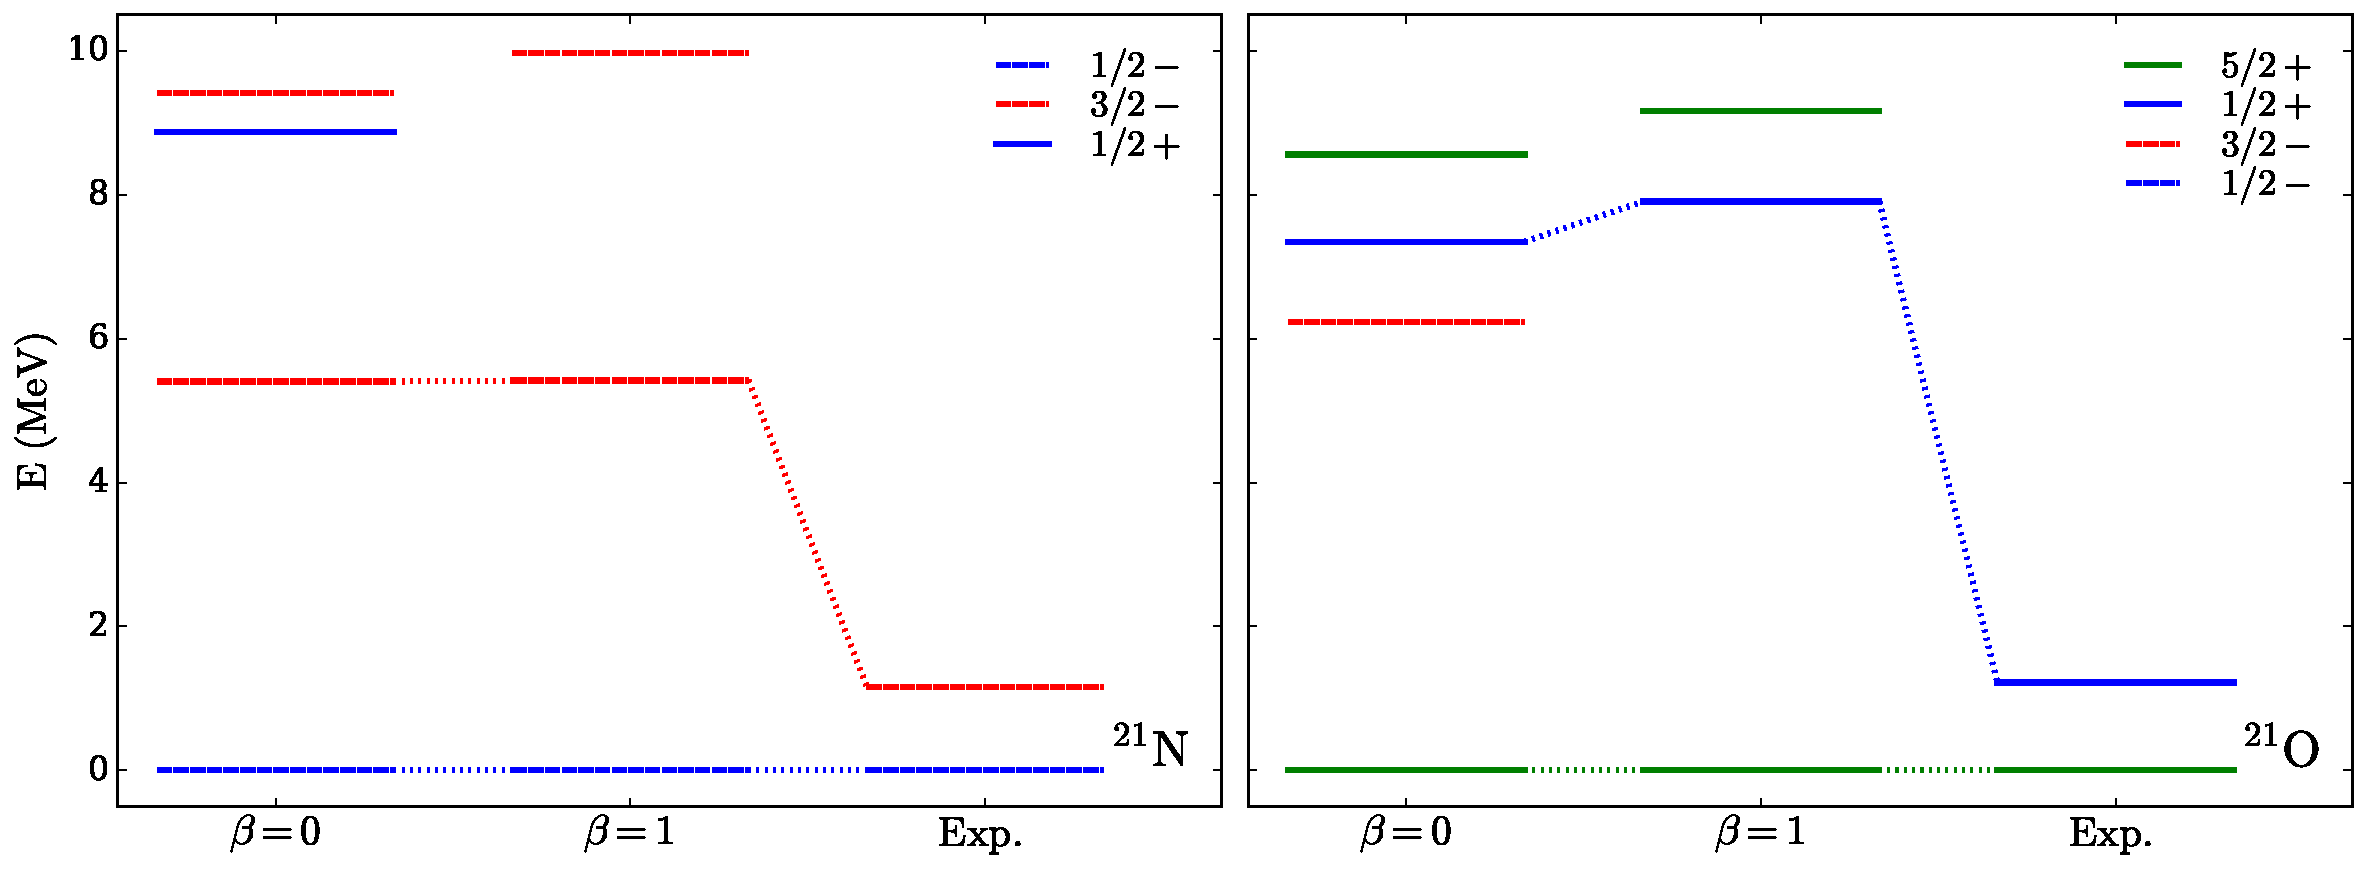
\includegraphics[width=\linewidth]{EOM/N21_O21_EOM_2.pdf}
  \caption{Low-lying PA-EOM states for $^{21}$N and $^{21}$O with and without a Lawson-Gloeckner term, Eq.\ \eqref{eq:lawson-term}, and the experimentally determined spectra. The negative-partiy states in $^{17}$O are COM contaminants and are removed by artificially raising the COM excitation energy.  The excited states of these nuclei have not been experimentally detemined.}
  \label{fig:N21O21_spectra}
\end{figure}

While the experimental excited states of the particle-attached nuclei $^{23}$O and $^{23}$F are not well-known, the EOM states can be treated in an equivalent way to remove the negative-parity states in $^{23}$O, shown in Fig. \ref{fig:O23F23_spectra}.  The low-lying excited states of the particle-removed nuclei $^{15}$N and $^{15}$O are shown in Fig. \ref{fig:N15O15_spectra} and those of $^{21}$N and $^{21}$O are shown in Fig. \ref{fig:N21O21_spectra}.  These EOM-CC states can now be used to calculate properties of excited-states and open-shell systems.  In particular, the transition amplitudes between neutron- and proton-attached states, or between neutron- and protron-removed states, describes the nuclear structure components of the corresponding beta-decay.

\end{document}
